\documentclass[]{article}
\usepackage{lmodern}
\usepackage{amssymb,amsmath}
\usepackage{ifxetex,ifluatex}
\usepackage{fixltx2e} % provides \textsubscript
\ifnum 0\ifxetex 1\fi\ifluatex 1\fi=0 % if pdftex
  \usepackage[T1]{fontenc}
  \usepackage[utf8]{inputenc}
\else % if luatex or xelatex
  \ifxetex
    \usepackage{mathspec}
    \usepackage{xltxtra,xunicode}
  \else
    \usepackage{fontspec}
  \fi
  \defaultfontfeatures{Mapping=tex-text,Scale=MatchLowercase}
  \newcommand{\euro}{€}
\fi
% use upquote if available, for straight quotes in verbatim environments
\IfFileExists{upquote.sty}{\usepackage{upquote}}{}
% use microtype if available
\IfFileExists{microtype.sty}{%
\usepackage{microtype}
\UseMicrotypeSet[protrusion]{basicmath} % disable protrusion for tt fonts
}{}
\usepackage[margin=1in]{geometry}
\usepackage{longtable,booktabs}
\usepackage{graphicx}
\makeatletter
\def\maxwidth{\ifdim\Gin@nat@width>\linewidth\linewidth\else\Gin@nat@width\fi}
\def\maxheight{\ifdim\Gin@nat@height>\textheight\textheight\else\Gin@nat@height\fi}
\makeatother
% Scale images if necessary, so that they will not overflow the page
% margins by default, and it is still possible to overwrite the defaults
% using explicit options in \includegraphics[width, height, ...]{}
\setkeys{Gin}{width=\maxwidth,height=\maxheight,keepaspectratio}
\ifxetex
  \usepackage[setpagesize=false, % page size defined by xetex
              unicode=false, % unicode breaks when used with xetex
              xetex]{hyperref}
\else
  \usepackage[unicode=true]{hyperref}
\fi
\hypersetup{breaklinks=true,
            bookmarks=true,
            pdfauthor={},
            pdftitle={Example},
            colorlinks=true,
            citecolor=blue,
            urlcolor=blue,
            linkcolor=magenta,
            pdfborder={0 0 0}}
\urlstyle{same}  % don't use monospace font for urls
\setlength{\parindent}{0pt}
\setlength{\parskip}{6pt plus 2pt minus 1pt}
\setlength{\emergencystretch}{3em}  % prevent overfull lines
\setcounter{secnumdepth}{0}

%%% Use protect on footnotes to avoid problems with footnotes in titles
\let\rmarkdownfootnote\footnote%
\def\footnote{\protect\rmarkdownfootnote}

%%% Change title format to be more compact
\usepackage{titling}

% Create subtitle command for use in maketitle
\newcommand{\subtitle}[1]{
  \posttitle{
    \begin{center}\large#1\end{center}
    }
}

\setlength{\droptitle}{-2em}
  \title{Example}
  \pretitle{\vspace{\droptitle}\centering\huge}
  \posttitle{\par}
  \author{}
  \preauthor{}\postauthor{}
  \date{}
  \predate{}\postdate{}



\begin{document}

\maketitle


{
\hypersetup{linkcolor=black}
\setcounter{tocdepth}{2}
\tableofcontents
}
\listoffigures

\listoftables
\newpage

\section{Introduction}\label{introduction}

This is an example of an RMarkdown document that can be authored using
\texttt{compileRmd}.\\The html version was compiled using the command:
\texttt{compileRmd()}.\\The word version was compiled using:
\texttt{compileRmd(format=\textquotesingle{}word\textquotesingle{})}.\\The
pdf version was compiled using:
\texttt{compileRmd(format=\textquotesingle{}tex\textquotesingle{}, texEngine=\textquotesingle{}pdflatex\textquotesingle{}, bibEngine=\textquotesingle{}bibtex\textquotesingle{})}.

\subsection{Motivation}\label{motivation}

I use RMarkdown for most of my writing.

It is missing some features, such as the ability to number figures (or
tables) and then cross-referencing them later. So, I thought I'd try
coming up with a way of adding this feature.

At the same time, I was also interested in getting a better handle on
regular expressions, and this problem gave me an excuse to play with
them. Conventional wisdom would suggest this was a bad idea:

\begin{quote}
Some people, when confronted with a problem, think ``I know, I'll use
regular expressions.''\\Now they have two problems.\\-
\href{http://en.wikiquote.org/wiki/Jamie_Zawinski}{jwz}
\end{quote}

I've tried to avoid using long, intricate regexs because:

\begin{enumerate}
\item
  I didn't want the source code to look like it was written by
  \href{http://en.wikipedia.org/wiki/Q*bert}{Q*bert}\\
\item
  I'm not \emph{that} good at regex to begin with
\end{enumerate}

\section{Basics}\label{basics}

\subsection{YAML Headers}\label{yaml-headers}

The YAML header contains information which RMarkdown and Pandoc use for
producing the output. It is usually the first thing in an Rmarkdown
document.

An example of a basic YAML header for tex (pdf) output is below:

\begin{verbatim}
---
output:
  pdf_document:
    fig_caption: yes
    keep_tex: yes
bibliography: [`varBib`]
csl: `varCSL`
---
\end{verbatim}

The bare minimum file structure for `compileRmd' is an RMarkdown .Rmd
file which contains a YAML header for either an html, word or pdf
document. However, this is not the most practical way because the YAML
header specifies the output format. So, if you want to output a pdf and
docx file, you'd have to change the YAML header. An alternative is to
split the YAML header into an external file, and save it as either
\texttt{yaml\_md.txt}, \texttt{yaml\_html.txt},
\texttt{yaml\_htmlB.txt}, \texttt{yaml\_word.txt}, or
\texttt{yaml\_tex.txt}. When we're outputting to a format, such as html,
we can make \texttt{compileRmd} grab the html header without having to
do anything ourselves. If the above naming scheme is used, then
\texttt{compileRmd} will automatically read the header file. Otherwise,
you will have to specify the file using
\texttt{compileRmd(yaml=\textquotesingle{}path/to/yaml\_header.txt\textquotesingle{})}

Another advantage of having YAMl headers as separate files is that each
output format can have its own settings without conflicting with each
other. Beyond this, additional files such as templates or .bib files can
also be included in the YAML header.

Look through the YAML files (\texttt{yaml\_*.txt}) which are in the same
folder as this .Rmd file. You'll see that the .bib file has been
included in the YAMl header, and there are also some knitr settings. For
example, the html YAML has a style.css and has PNG output for figures,
whereas the tex YAML has pdf output for figures.

Additionally, some parts of the YAMl header contain placeholders such as
\texttt{varBib} and \texttt{varCSL}, which are placeholders for the .bib
and .csl files respectively. The input arguments (e.g.
\texttt{compileRmd(bibFile=\textquotesingle{}path/to/file.bib\textquotesingle{}, cslFile=\textquotesingle{}path/to/file.csl\textquotesingle{})})
will overwrite the placeholder. Alternatively, the user can enter the
appropriate files into the YAML header directly. In this example's
headers, the .bib file is specified in the YAML header, but the csl file
is not.

\subsection{Syntax}\label{syntax}

Markdown's syntax is straightforward so it should be easy to pick up by
just reading the source document.

Perhaps the only thing that might leave newcomers confused is how to
force a line break.\\Simply hitting the\\enter key will not cause a\\new
line to begin.\\The previous sentence is broken into lines (it might
qualify as a haiku?) yet the 2nd last sentence is not broken. The
reasoning is subtle: you need two blank spaces before breaking the line
to create a new line.

\subsection{Citations}\label{citations}

Here, look, it's a citation to a fictional paper \cite{Rosencrantz}.

For html or word output, pandoc's citation syntax can also be used. This
becomes a bit troublesome if the desired output format is \emph{not}
LaTeX because it will hardcode the .tex output by default. There's a
special document for details.

\subsection{Equations}\label{equations}

An in-line equation can be dropped, \(f(x) = \sqrt{(ax - b)^2}\),
anywhere. The syntax is identical to LaTeX, and c\(\alpha\)n
b\(\epsilon\) use\(\delta\) for symbols as well.

Some equations are important and deserve their own block. For example,
the following equation keeps me up at night: \[
P(job|degree) = \frac{P(degree|job) P(job)}{P(degree)}
\]

More often than not, equations have to be referenced in the text. One
way to do this is by numbering them. For example, equation
\ref{eq:cDonald} is the well known cDonald's theorm.
\begin{equation} \label{eq:cDonald}
n^2 + 9 + 9
\end{equation}
\subsection{Figures and Images}\label{figures-and-images}

Have a look at figure \ref{fig:LifeOfSWE}. It contains a short caption
which will not show up in the figure caption, but will show up in the
list of figures (pdf output only).

\begin{figure}[htbp]
\centering
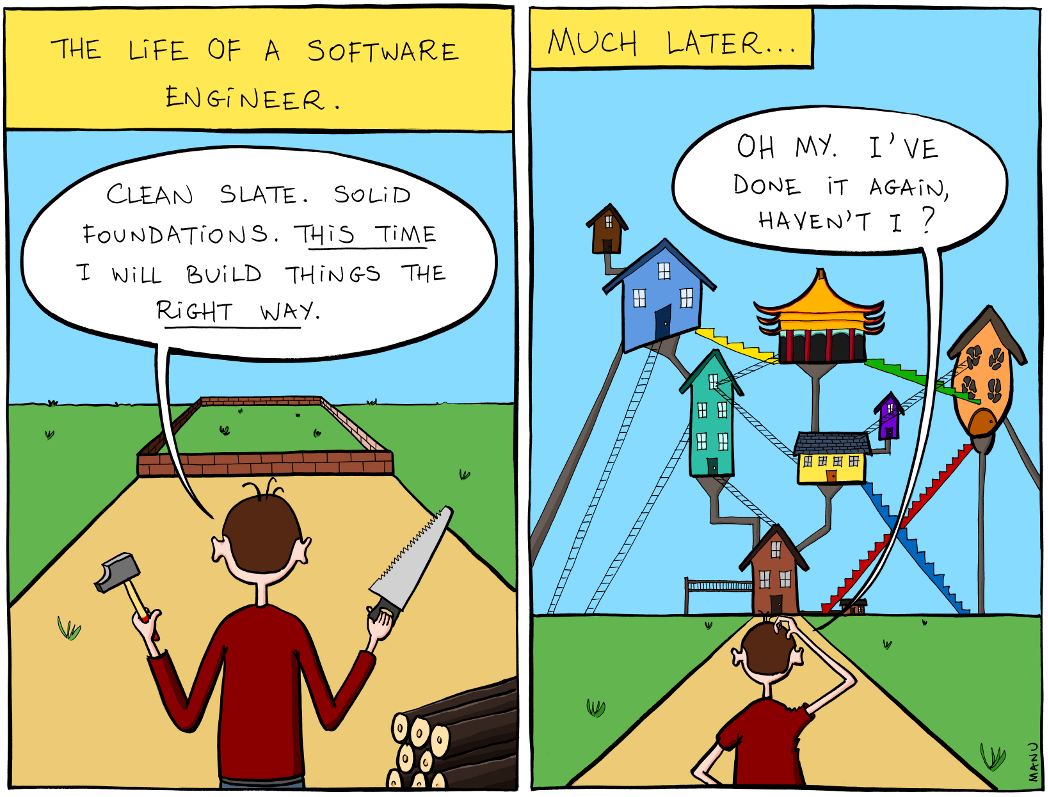
\includegraphics{imgs/manu-LifeOfSWE.png}
\caption[Comic: Life of a software engineer]{ Is this what people
mean when they say `building code violations'?
Artist:\href{http://www.bonkersworld.net/building-software/}{Manu
Cornet} \label{fig:LifeOfSWE}}
\end{figure}

\subsection{Tables}\label{tables}

I have a habit of avoiding tables because they're usually a pain to make
- for example, tables in LaTeX require a summoning ritual which I can
never get quite right on the first try. Thankfully, tables are pretty
easy to make in Markdown. Check out table \ref{tab:fiction} below.

\begin{longtable}[c]{@{}cc@{}}
\caption[Simple table]{ A fictional table. Chairs not included.
\label{tab:fiction}}\tabularnewline
\toprule
x & y\tabularnewline
\midrule
\endfirsthead
\toprule
x & y\tabularnewline
\midrule
\endhead
1 & 1\tabularnewline
2 & 4\tabularnewline
3 & 9\tabularnewline
4 & 16\tabularnewline
\bottomrule
\end{longtable}

The next chapter will show an even easier way of making tables.

\section{Dynamic Results}\label{dynamic-results}

It is possible to embed code in a RMarkdown file and have it execute
when the output is produced. This chapter provides an example of that.

\subsection{Tables}\label{tables-1}

I have a csv file saved in the \texttt{./exampleData/} folder which
contains a summary of the New York vs Washington series of the
\href{http://en.wikipedia.org/wiki/2015_Stanley_Cup_playoffs\#.28M1.29_New_York_Rangers_vs._.28M2.29_Washington_Capitals}{2015
Stanley Cup Playoffs}. The CSV only contains the goals scored by each
team. We can calculate the goal difference, and the win/loss through R,
and display the results. Check out table \ref{tab:NYRvsWSH} which shows
the results.

\begin{longtable}[c]{@{}ccccc@{}}
\caption[Summary of NYR vs WSH]{ Summary of New York Rangers vs
Washington Capitals series of the 2015 Stanley Cup Playoffs, from the
Rangers POV \label{tab:NYRvsWSH}}\tabularnewline
\toprule
Game & Goals For & Goals Against & Goal Diff & Win - Loss\tabularnewline
\midrule
\endfirsthead
\toprule
Game & Goals For & Goals Against & Goal Diff & Win - Loss\tabularnewline
\midrule
\endhead
1 & 1 & 2 & -1 & 0 - 1\tabularnewline
2 & 3 & 2 & +1 & 1 - 1\tabularnewline
3 & 0 & 1 & -1 & 1 - 2\tabularnewline
4 & 1 & 2 & -1 & 1 - 3\tabularnewline
5 & 2 & 1 & +1 & 2 - 3\tabularnewline
6 & 4 & 3 & +1 & 3 - 3\tabularnewline
7 & 2 & 1 & +1 & 4 - 3\tabularnewline
\bottomrule
\end{longtable}

\subsection{Analysis}\label{analysis}

Let's perform some simple analysis on the data in table
\ref{tab:NYRvsWSH}.

The New York Rangers scored a total of 13 goals, with an average of 1.9
\(\pm\) 1.3 goals per game. The highest scoring game for the Rangers was
game 6 where they scored 4 goals. This was a hard-fought series, but
ultimately won by the \textbf{New York Rangers}.

If you're reading the output document, then the previous paragraph
probably looks normal (asside from the obnoxious bold at the end). In
the .Rmd source, you can see that there is embedded R code. For
tidiness, I did the calculations inside an R code block, and then called
the results in-line. The advantage with this is that these results will
automatically change if the input data was changed.

For example, suppose that the csv data was incorrect and that game 7
actually had 5 goals scored in favour of New York and 8 goals scored by
Washington. This means that table \ref{tab:NYRvsWSH} has to be changed.
Furthermore, the results of our analysis (the total goals, average goals
per game, highest scoring game, and the eventual winner) will all have
to be changed. That's a lot of work\ldots{} but not for us - all we have
to do is update the CSV file.

To test this, I modified the csv file and saved it as
\texttt{./exampleData/NYRvsWSH-alt.csv}. Change the `Load Data' line in
the R code above to read this csv file and re-compile this document to
see the results.

\subsection{Figures}\label{figures}

Figures can also be created at runtime and embedded. Take a look at
figure \ref{fig:NYRvsWSH-Goals}. This figure will also change if the csv
data changes.

\begin{figure}[htbp]
\centering
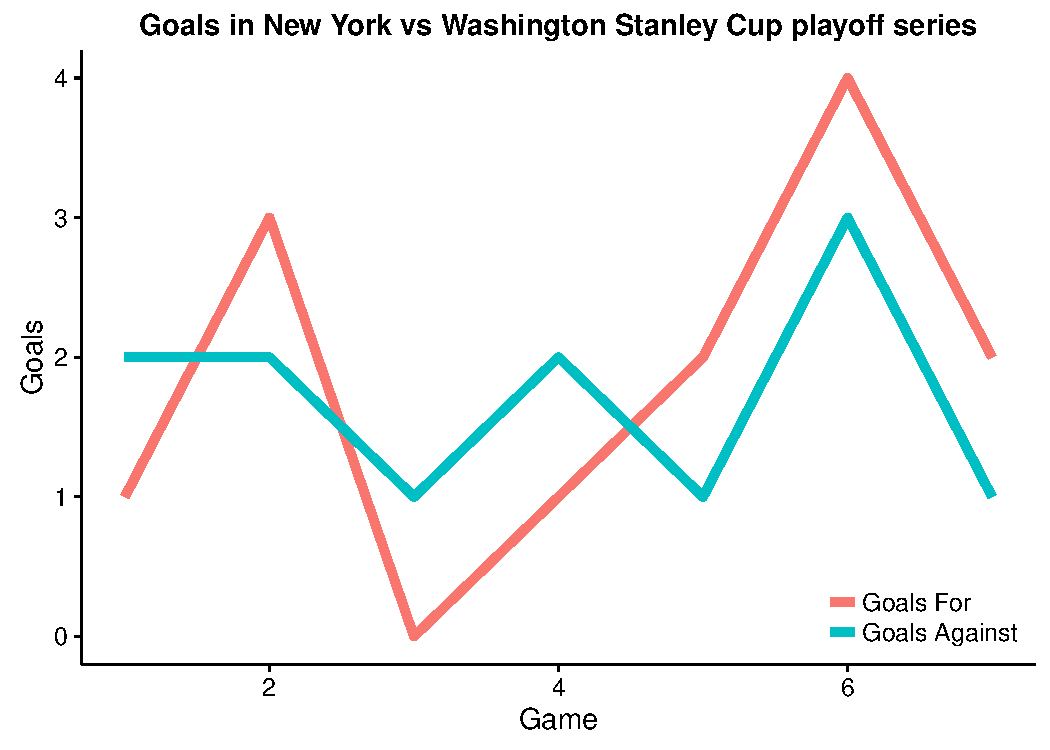
\includegraphics{figure/NYRvsWSH-Fig-1.pdf}
\caption[Goals for NYR vs WSH]{ Goals in the New York vs Washington
series. \label{fig:NYRvsWSH-Goals}}
\end{figure}

\section{References}\label{references}

\ifdefined\chapter  
\renewcommand{\chapter}[2]{}  
\else  
\renewcommand{\section}[2]{}  
\fi  
\bibliography{./bib/refsA.bib}
\bibliographystyle{plain}
\end{document}
